\subsection{LaCuerda}
LaCuerda\cite{lacuerdanet_home} es una aplicación web dedicada principalmente a la guitarra, aunque también ofrece soporte para otros instrumentos como el ukelele, el piano, el charango y la armónica. Entre las páginas que componen la aplicación distinguimos las relacionadas con canciones, herramientas y las informativas.

En primer lugar, con respecto a las \textbf{páginas relacionadas con canciones}, podemos encontrar:
\begin{itemize}
    \item \textbf{Biblioteca de canciones} (véase Figura~\ref{fig:lacuerdanet_home}), con la posibilidad de realizar búsquedas sencillas por artista o canción.
    \item \textbf{Canciones} (véase Figura~\ref{fig:lacuerdanet_somewhereovertherainbow}) que contienen la letra, acordes y utilidades (véase Tabla~\ref{tab:lacuerda_utilidades_canciones}) para la práctica de las mismas.
    \item \textbf{Solicitudes} de nuevas canciones.
\end{itemize}

En segundo lugar, en cuanto a las \textbf{páginas de herramientas e informativas}, podemos encontrar:
\begin{itemize}
    \item \textbf{Cursos} (véase Figura~\ref{fig:lacuerdanet_courses}) que incluyen lecciones en forma de artículos y vídeos, dedicados especificamente a aprender a tocar la guitarra. También encontramos algunas publicaciones enfocadas a otros instrumentos.
    \item \textbf{Diccionario de acordes} (véase Figura~\ref{fig:lacuerdanet_acordes}), que permite la búsqueda y visualización de acordes en un diagrama.
    \item \textbf{Afinador de instrumento interactivo}, haciendo uso del micrófono integrado en el dispositivo.
    \item \textbf{Biblioteca de rasgueos}, con pistas de audio.
\end{itemize}

\begin{figure}[H]
    \centering

    % Primera fila
    \begin{subfigure}[t]{0.48\textwidth}
         \centering
        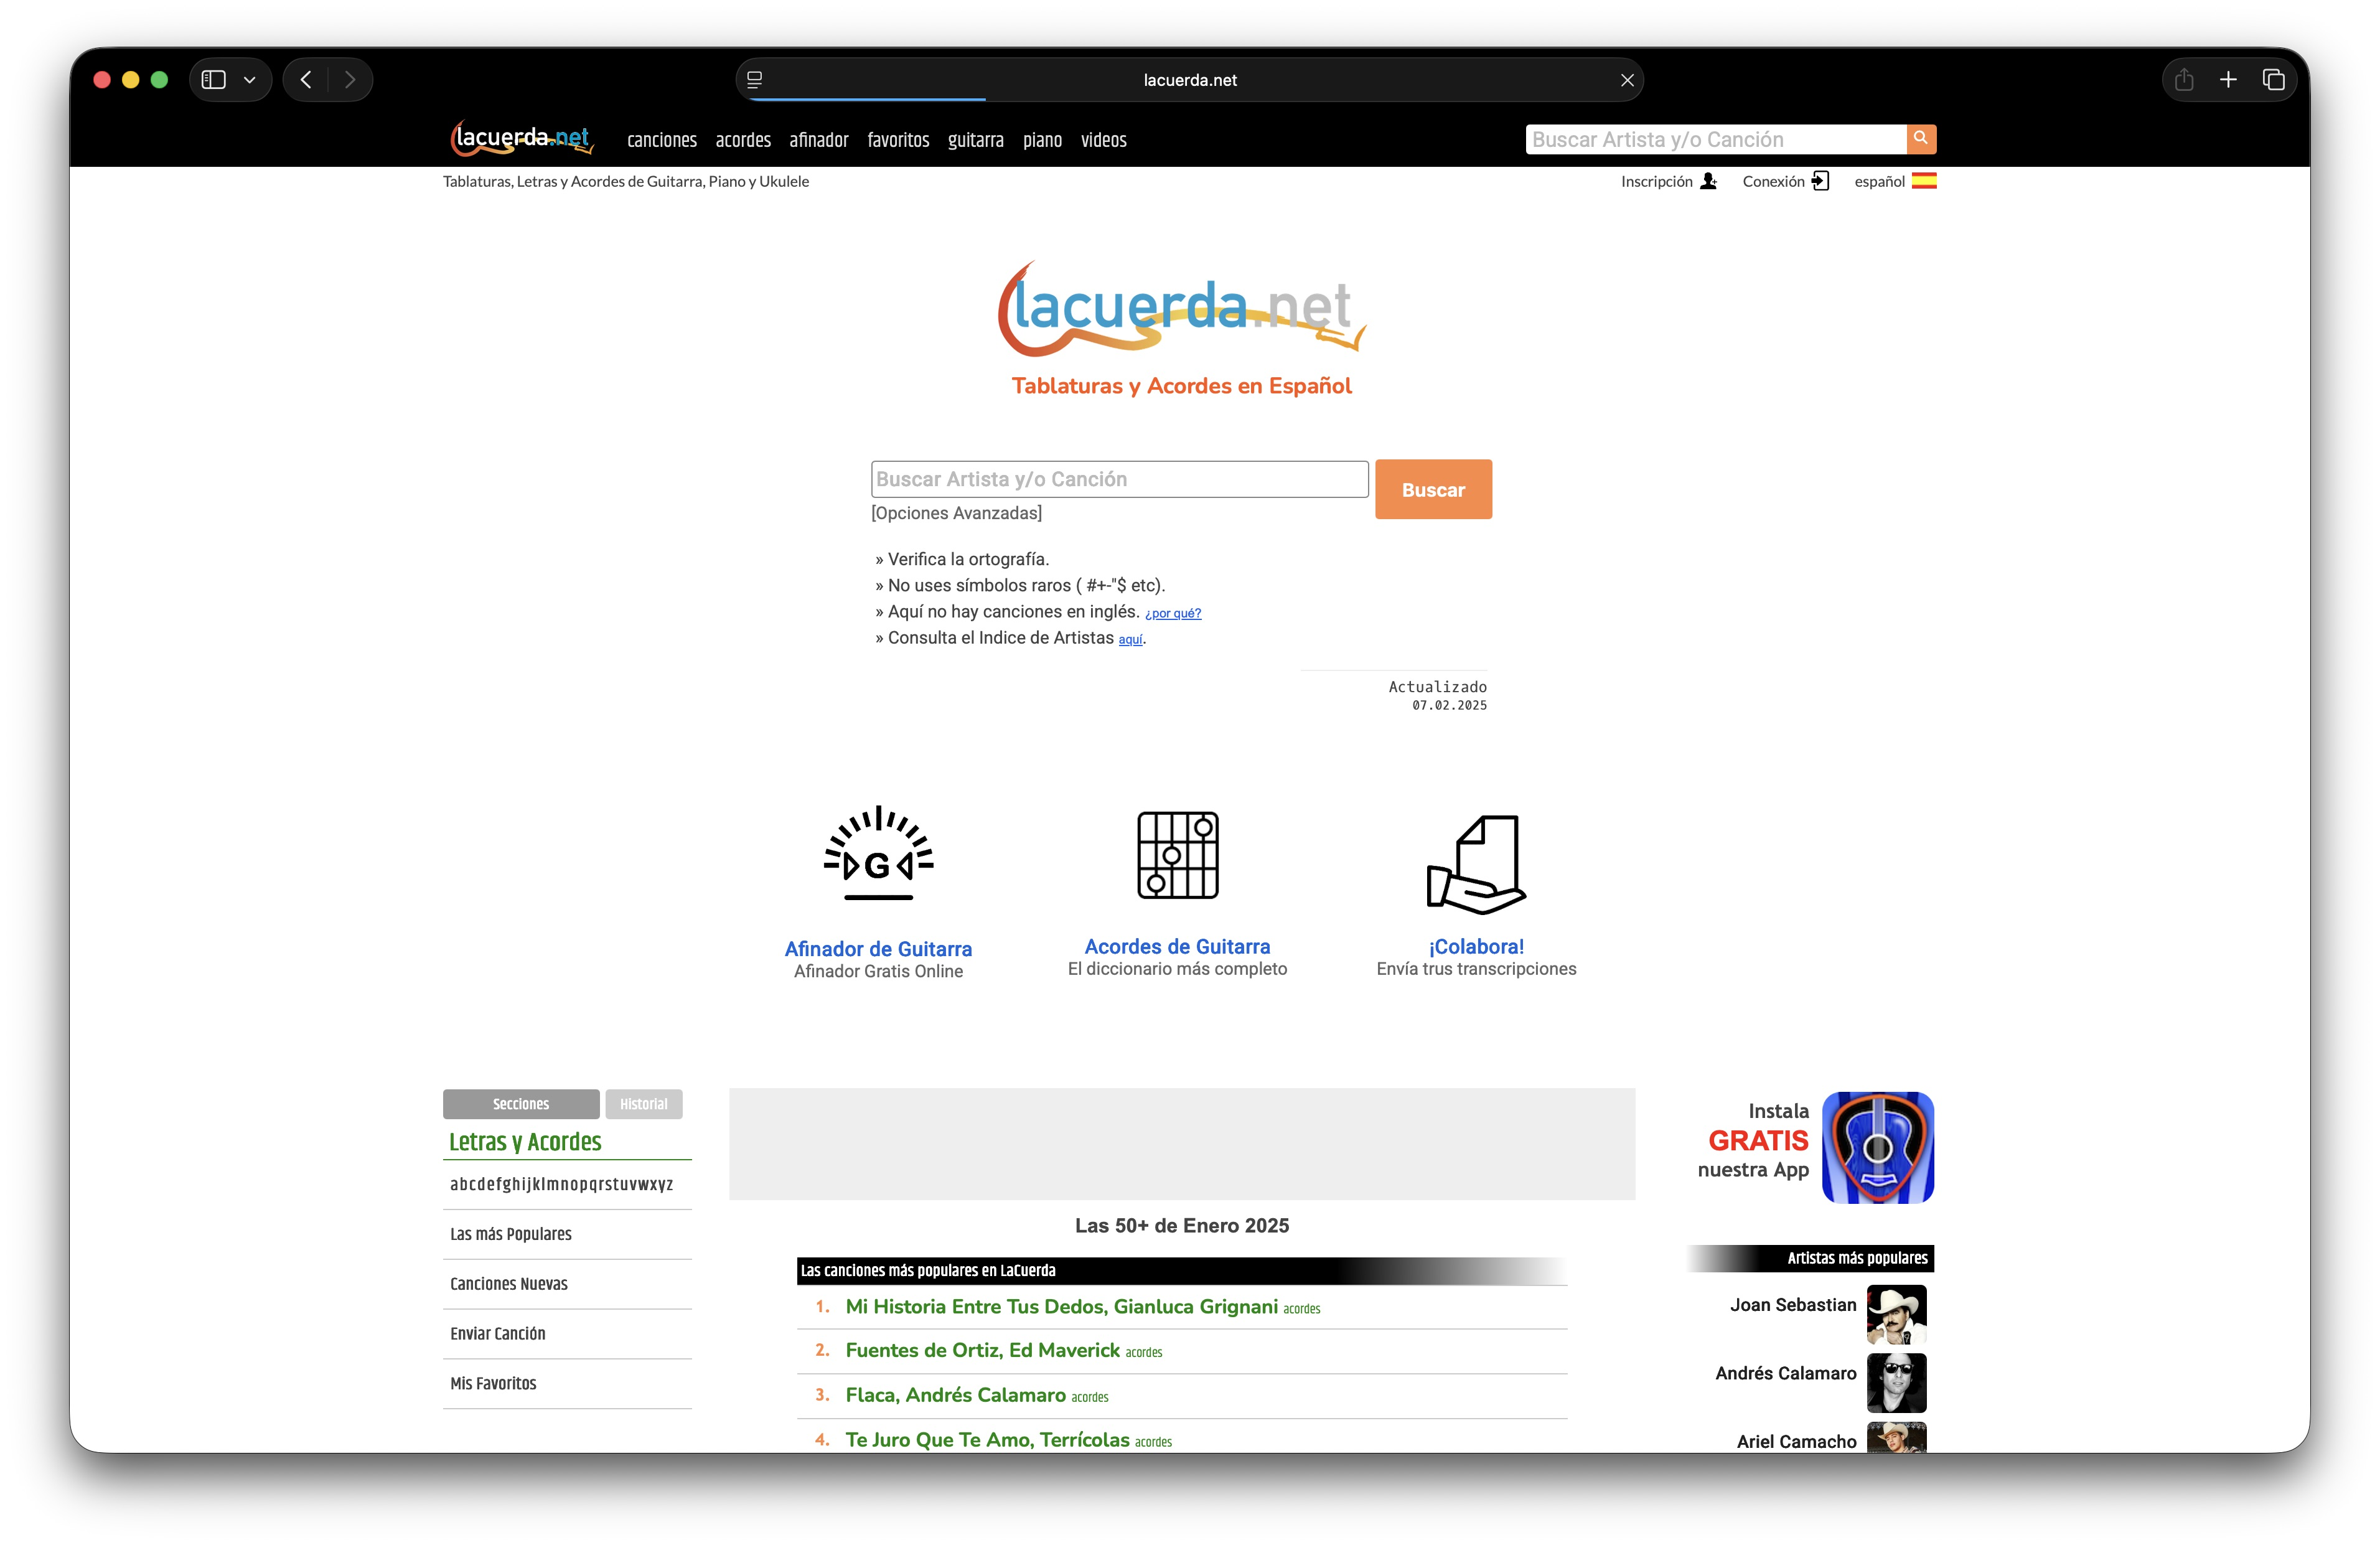
\includegraphics[width=\textwidth]{Ilustraciones/estado/lacuerdanet.jpeg}
        \caption{Página principal de LaCuerda~\cite{lacuerdanet_home}}\label{fig:lacuerdanet_home}
    \end{subfigure}
    \hfill
    \begin{subfigure}[t]{0.48\textwidth}
        \centering
        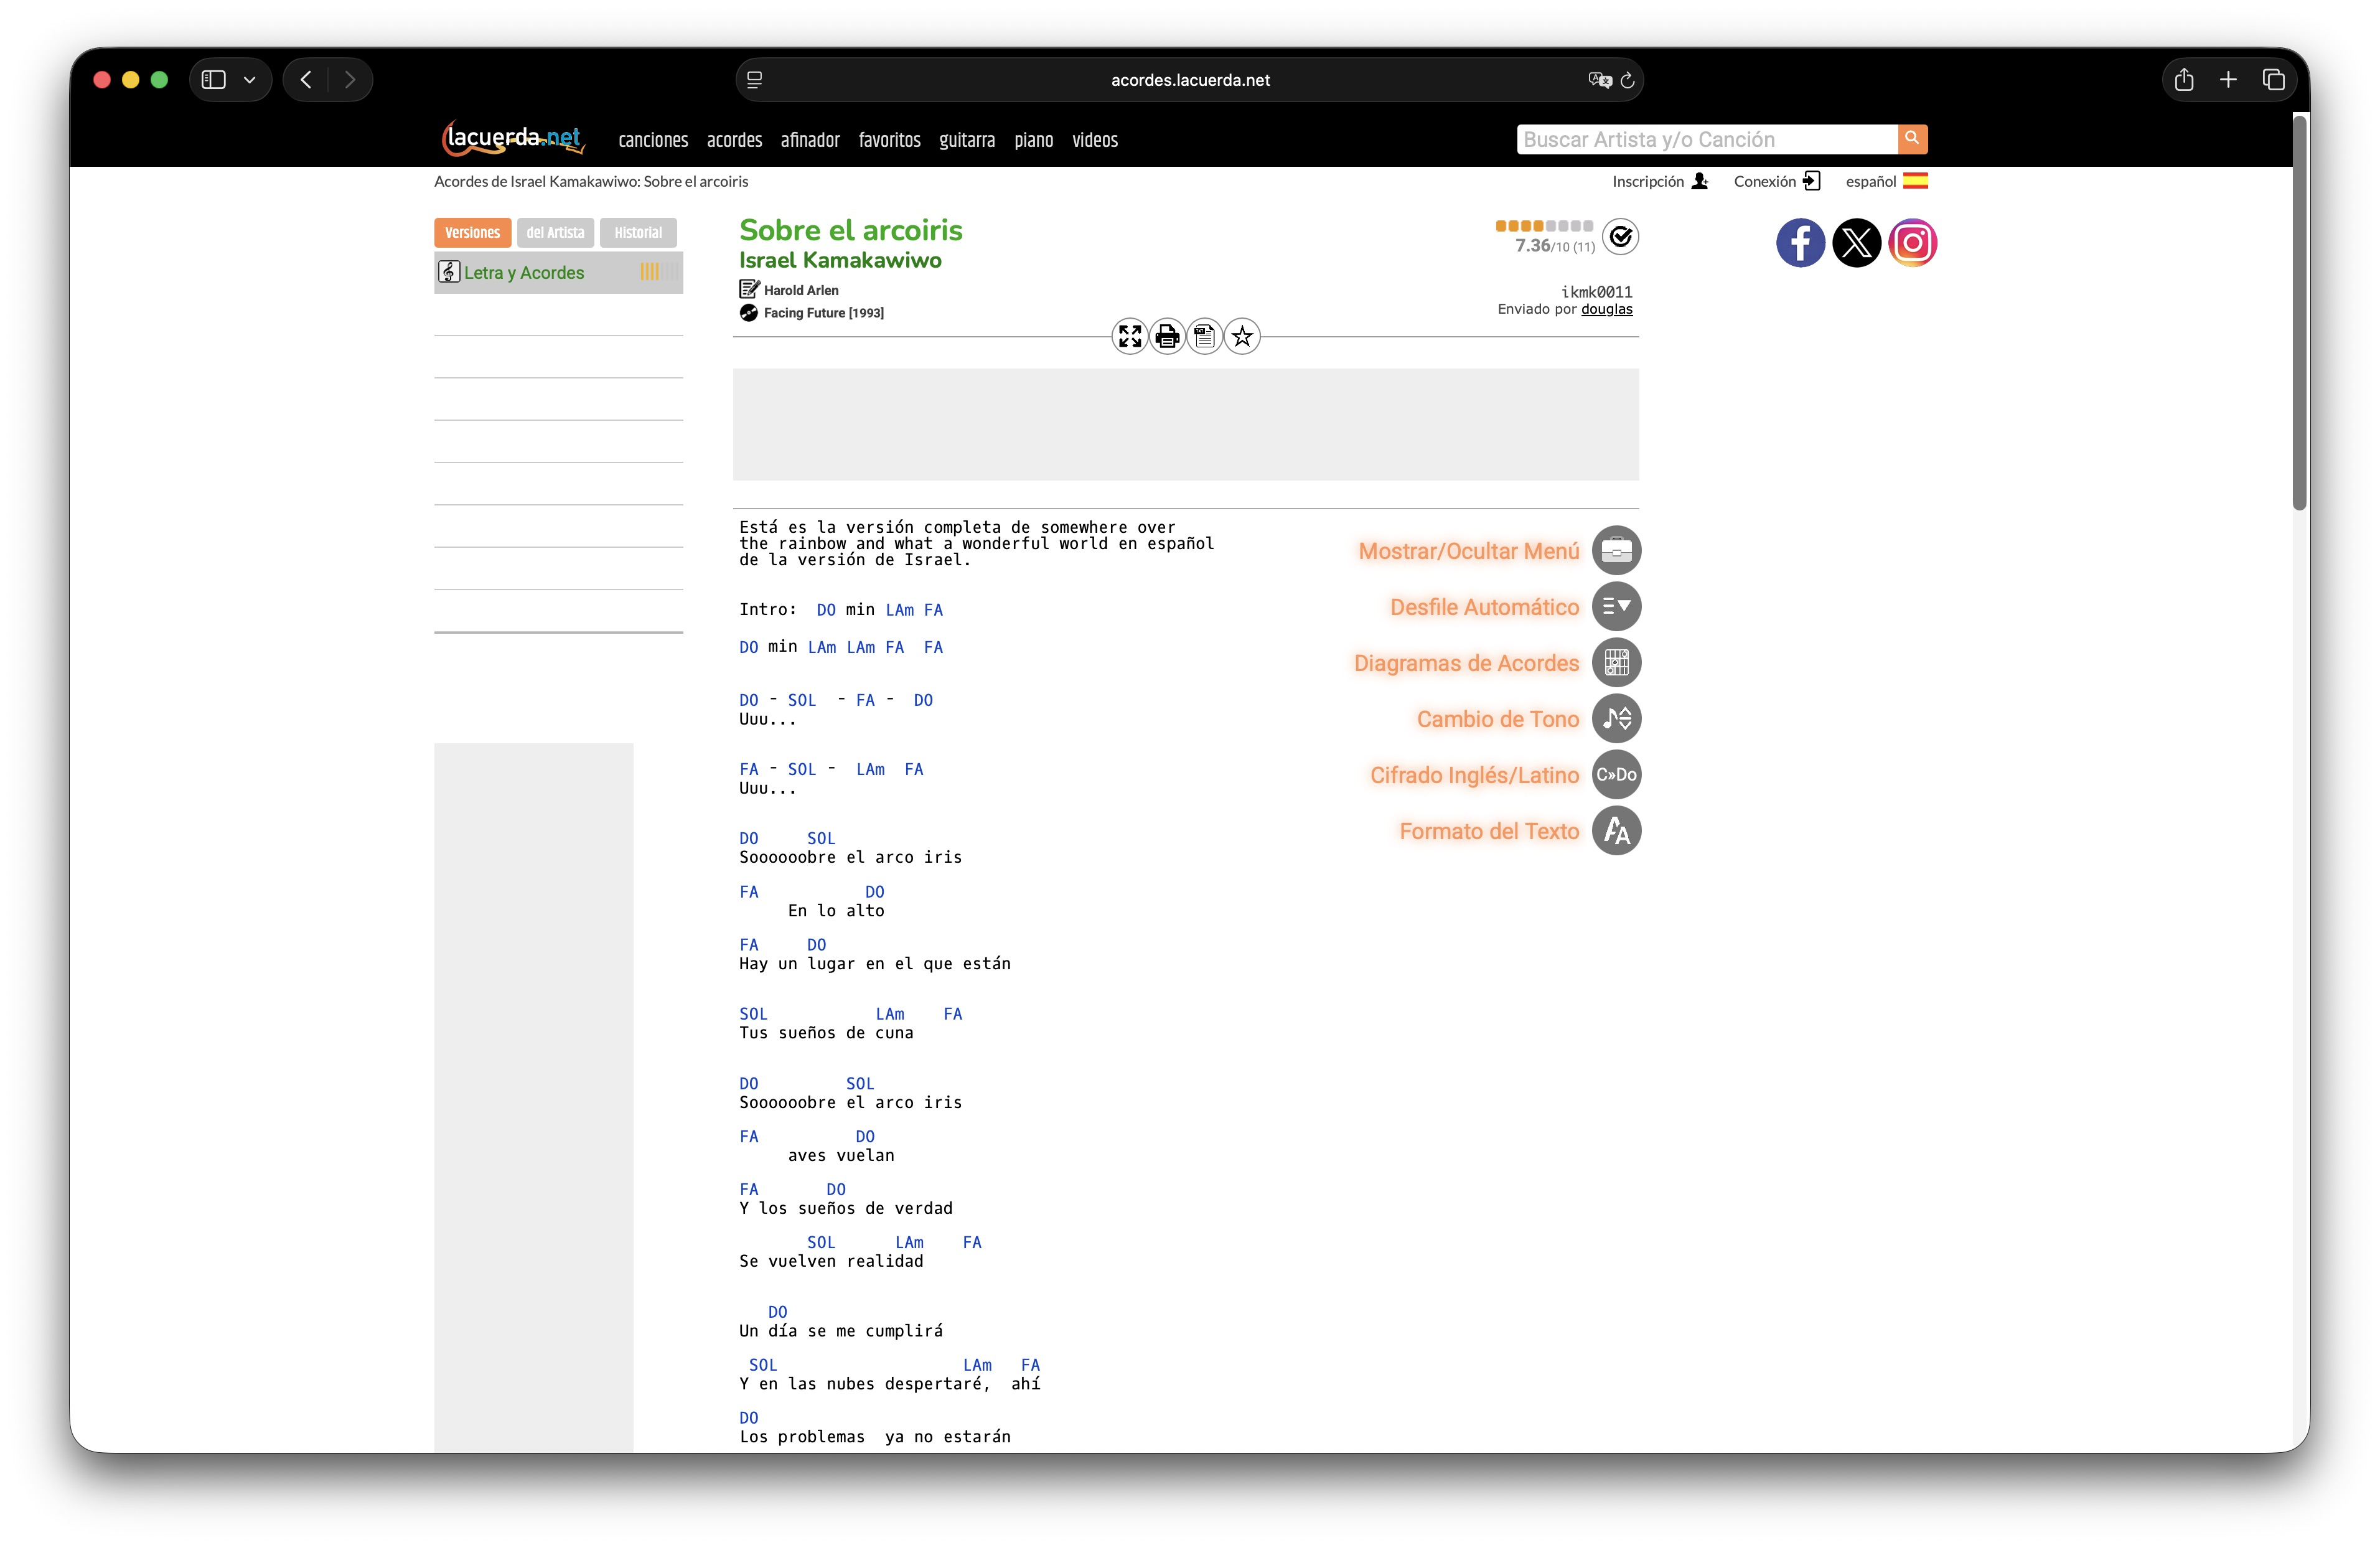
\includegraphics[width=\textwidth]{Ilustraciones/estado/lacuerdanet_somewhereovertherainbow.jpeg}
        \caption{Acordes y letra de \emph{Somewhere over the rainbow}~\cite{lacuerdanet_somewhereovertherainbow} para guitarra en LaCuerda}
        \label{fig:lacuerdanet_somewhereovertherainbow}
    \end{subfigure}
    \vspace{1em} % Espacio vertical entre filas

    % Segunda fila
    \begin{subfigure}[t]{0.48\textwidth}
        \centering
        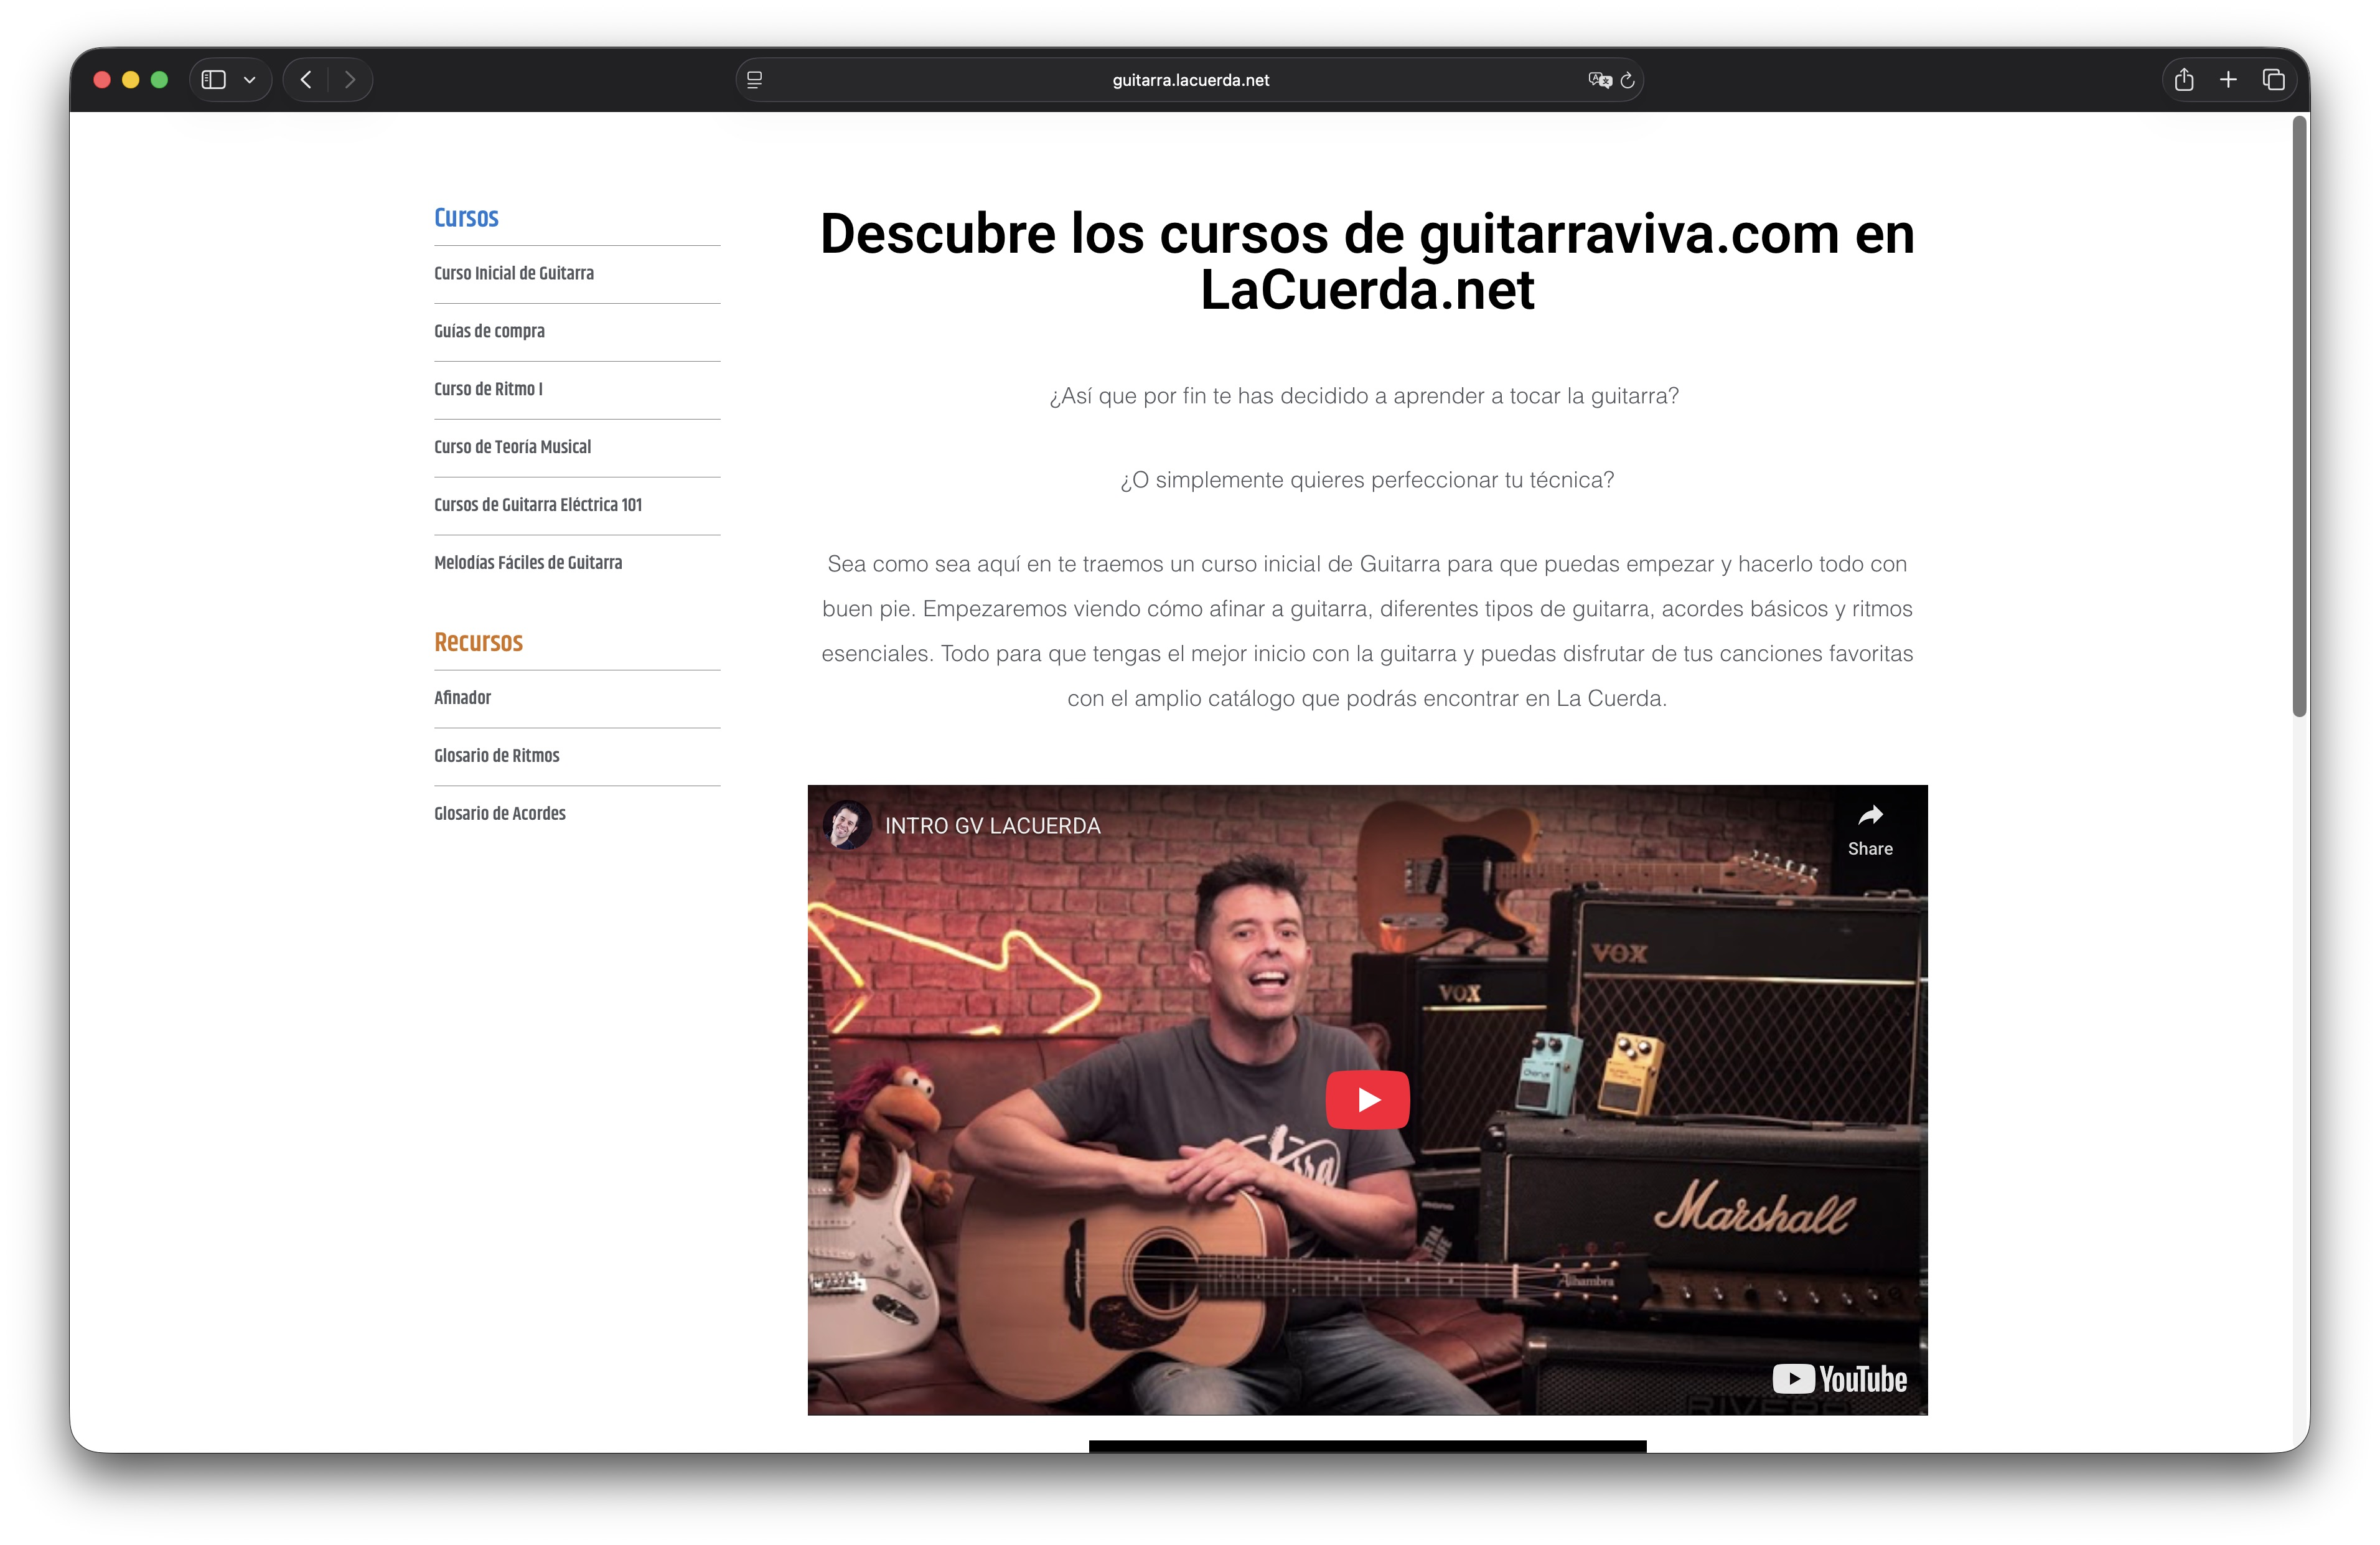
\includegraphics[width=\textwidth]{Ilustraciones/estado/lacuerdanet_cursos.jpeg}
        \caption{Página de cursos de LaCuerda~\cite{lacuerdanet_courses}}
        \label{fig:lacuerdanet_courses}
    \end{subfigure}
    \begin{subfigure}[t]{0.48\textwidth}
        \centering
        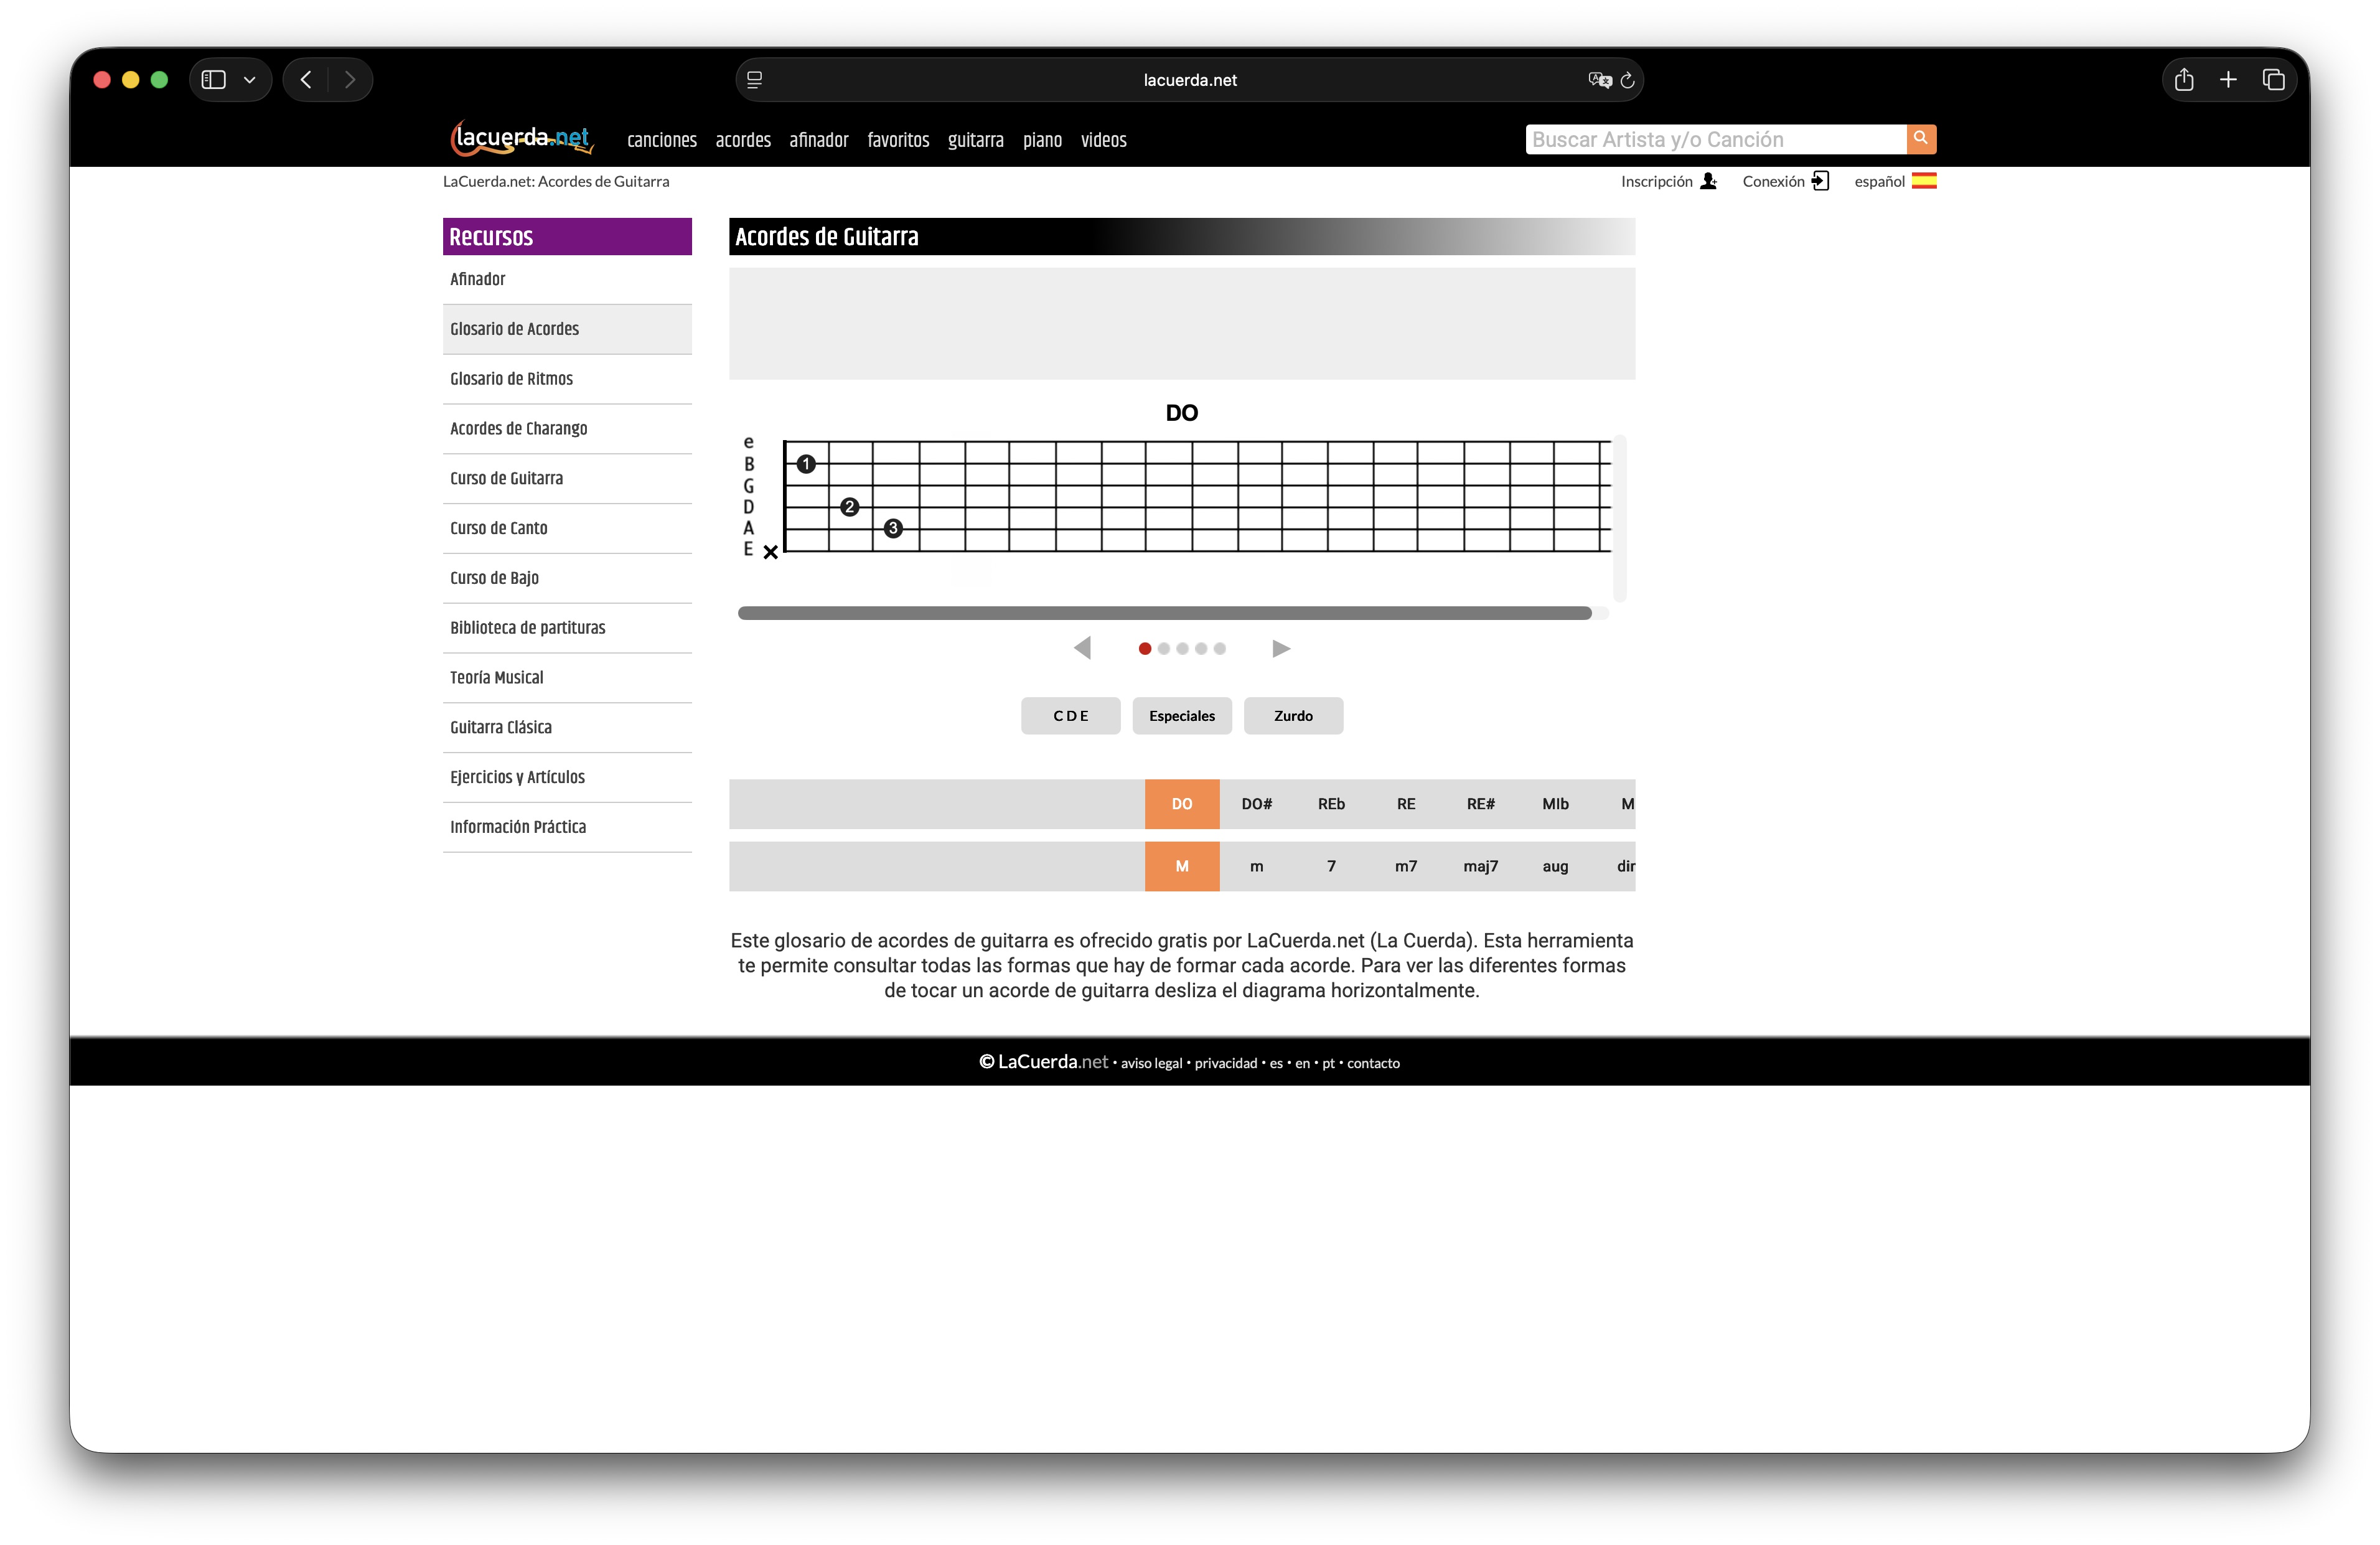
\includegraphics[width=\textwidth]{Ilustraciones/estado/lacuerdanet_acordes.jpeg}
        \caption{Página de cursos de LaCuerda~\cite{lacuerdanet_acordes}}
        \label{fig:lacuerdanet_acordes}
    \end{subfigure}

    \caption{Páginas de LaCuerda.}
    \label{fig:lacuerdanet_canciones}
\end{figure}

LaCuerda es en conclusión, una aplicación web que cuenta con una interfaz de apariencia anticuada en comparación con las otras alternativas analizadas, ofreciendo practicamente las mismas herramientas. No obstante, dada su antigüedad, dispone de un amplio catálogo de recursos, desde canciones hasta lecciones para aprender a tocar distintos instrumentos. A pesar de su método de verificación de contenido a través de administradores, podemos encontrar distintas versiones de una misma canción, incluso otorgándole autoría a los usuarios que realizan las aportaciones. Además, su modelo de negoció a través de anuncios permite el acceso gratuito a la mayoría de sus funcionalidades, incluso sin registro previo (véase Tabla~\ref{tab:lacuerda_funcionalidades_usuario}).

\begin{table}[H]
    \scriptsize
    \begin{minipage}[t]{0.4\textwidth}
    \centering
    \caption{Utilidades presentes en publicaciones de LaCuerda}\label{tab:lacuerda_utilidades_canciones}
    \begin{tabular}{l c}
        \hline
        \textbf{Utilidad} & \textbf{Existe} \\
        \hline
        Transportador & \ding{51} \\
        Lista de acordes & \ding{51} \\
        Autodesplazamiento & \ding{51} \\
        Impresión/Descarga & \ding{51} \\
        Cambio de notación & \ding{51}  \\
        Cambio de instrumento & \ding{51}  \\
        Guardar canción & \ding{51} \\
        Guía de rasgueos & \\
        \hline
    \end{tabular}
    \end{minipage}
\hfill
\begin{minipage}[t]{0.56\textwidth}
    \centering
    \caption{Funcionalidades disponibles según el rol del usuario de LaCuerda}\label{tab:lacuerda_funcionalidades_usuario}
    \begin{tabular}{l c c }
        \hline
        \multirow{2}{*}{\textbf{Funcionalidad}} & \multicolumn{2}{c}{\textbf{Rol Usuario}} \\
         & Visitante & Registrado \\
        \hline
        % --- Ejemplo de fila vacía (borra o completa) ---
        Biblioteca de canciones & \ding{51} & \ding{51} \\
        Creación y edición de publicaciones &  & \ding{51}  \\
        Utilidades de publicaciones & \ding{51} & \ding{51} \\
        Puntuar publicaciones &  & \ding{51}  \\
        Comentar publicaciones &  & \ding{51}  \\
        Solicitar nuevas canciones &  & \ding{51}  \\
        Cursos y guías & \ding{51} & \ding{51} \\
        Afinador & \ding{51} & \ding{51}  \\
        Calculadora de escalas y notas & &  \\
        Diccionario de acordes & \ding{51} & \ding{51}  \\
        % ------------------------------------------------
        \hline
    \end{tabular}
\end{minipage}
\end{table} 
